\section{Marco teórico} \label{marco_teorico}

\subsection{Potencial evocado auditivo}

El potencial evocado auditivo es una señal eléctrica generada por el nervio auditivo y distintas partes del encéfalo en respuesta a un estímulo sonoro. Una representación diagramática de un potencial evocado auditivo típico se muestra en la Figura \ref{fig:AEP}. La respuesta del tronco encefálico (ABR) corresponde con los primeros 10 ms, abarcando las ondas I a VI.

\begin{figure}[H]
    \centering
    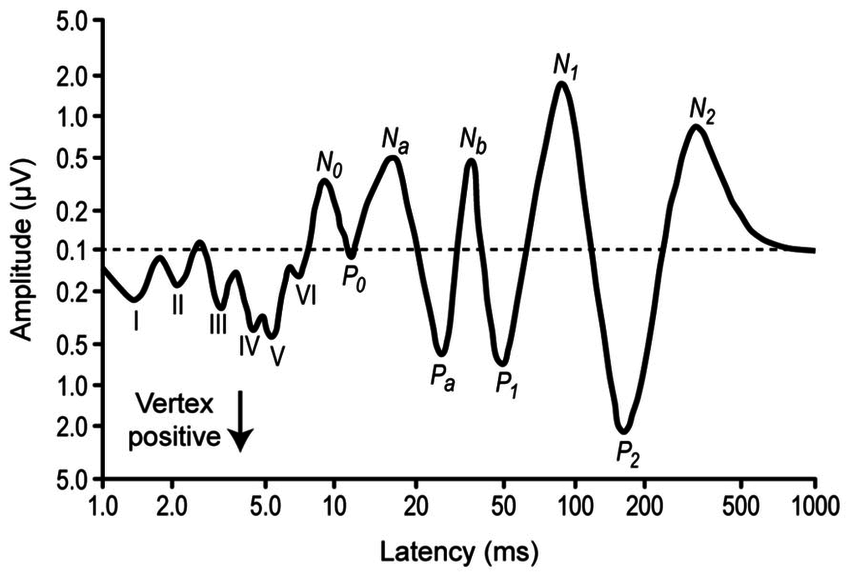
\includegraphics[width=0.8\linewidth]{figuras/AEP.png}
    \caption{Representación del potencial evocado auditivo. Como tal, este gráfico es ideal y no se observa con esta calidad en estudios clínicos. Obtenido de \cite{perez-gonzales-2014}.}
    \label{fig:AEP}
\end{figure}

Las mediciones principales que se realizan sobre el ABR son las latencias, amplitudes y duración de intervalos de las ondas I a III, III a V, y I a V. La latencia se define como el tiempo transcurrido entre que se aplica el estímulo y el pico de una onda. Tanto latencias como amplitudes son afectadas por la edad (mayor edad es igual a mayor latencia y menor amplitud) y la intensidad del estímulo (mayor intensidad es igual a menor latencia y mayor amplitud) \cite{young-ABR}.

Más allá de la tipificación del ABR, la presencia de estos marca que el estímulo sonoro efectivamente causó una respuesta neurofisiológica. Se define como umbral auditivo como la intensidad mínima a partir de la cual un ABR reproducible puede formarse y detectarse \cite{sininger-1993-ABR}.

No obstante, la percepción sonora puede verse afectada por patologías con incidencia en estructuras superiores, tales como el tálamo o la corteza. Esto no quita valor a la evaluación audiométrica a través de ABR. Al contrario, permite discernir con mayor granularidad cuáles son las patologías potenciales que pueden estar afectando al paciente, ya que evalúan el procesamiento sonoro en un punto intermedio entre su recepción y percepción consciente. 

\subsection{Adquisición de la señal fisiológica}

Para obtener una señal de potencial evocado auditivo del tipo ABR, se deben
colocar tres electrodos en el paciente de la siguiente manera:

\begin{itemize}
    \item Electrodo de activo ($V_{in}^{+}$): en la frente del paciente.
    \item Electrodo de tierra ($V_{in}^{-}$): en la apófisis mastoides ipsilateral del paciente.
    \item Electrodo de referencia (neutro): en la apófisis mastoides contralateral del paciente.
\end{itemize}

La señal de ABR se obtiene midiendo la diferencia de potencial entre los electrodos $V_{in}^{+}$ y $V_{in}^{-}$, utilizando como referencia de acoplamiento eléctrico al electrodo neutro. Esta señal es particularmente ruidosa, y su amplitud es del orden de los 500 [nV]. Por ello, se la debe filtrar y amplificar analógicamente previo a su tratamiento digital \cite{shojaeemend_automated_2018}.

Se suele utilizar un filtro pasabandas de 150 a 3000 [Hz] para eliminar ruido de baja y alta frecuencia. Para amplificar, como se explica más adelante, se utiliza una combinación de circuitos integrados para lograr una ganancia total de entre 10000 y 500000.

\subsection{Preprocesamiento digital de la señal}

Una vez que se cuenta con la señal digital, es necesario preacondicionarla previo a procesarla si se desea obtener un análisis con significancia. La relación fisiológica de señal-ruido (SNR por \textit{Signal-to-Noise Ratio}) para el potencial evocado es de -20 dB, considerando que la amplitud estándar del EEG (electroencefalograma) es de 5 $\mu$V \cite{young-ABR} y la del ABR de 0.5 $\mu$V  \cite{bhattacharyya-ABR}. Debido a tal limitación, es importante remover lo más posible el ruido que induce la etapa de adquisición de la señal analógica y su digitalización.

Dado que se necesitan múltiples repeticiones de una misma prueba para obtener un potencial evocado, todo el procesamiento de la señal se realiza de forma \textit{offline}, es decir, con las señales almacenadas por completo en memoria.

Como primera etapa, se introduce usualmente un filtro digital de tipo IIR (de \textit{Infinite Impulse Response}) que se aplica en ambos sentidos para eliminar la pobre respuesta en fase que poseen este tipo de diseños. No obstante, requieren de un menor orden para lograr las mismas especificaciones en amplitud que filtros de tipo FIR (de \textit{Finite Imput Response}) \cite{madsen-2017-AverageEP}.

A continuación, se descartan las repeticiones que posean un umbral mayor a una referencia, para evitar artefactos introducidos por ECG (electrocardiografía) y EMG (electromiografía). El umbral suele asignarse entre 25 y 40 $\mu$V.

\subsection{Obtención del potencial evocado}

Finalmente, se procede a realizar promediación por bloques. Este tipo de procesamiento asume que el ruido es independiente de la señal y aleatorio, por lo que puede removerse si múltiples repeticiones se apilan unas sobre otras \cite{davila-1992-Weigthed-Average}. Existen diversos modelos para elegir los pesos que se aplican a cada iteración, que tienen en cuenta factores como la amplitud del ruido (estimado por la varianza de cada ensayo) y la señal (estimada como el producto punto entre el promedio y cada iteración) \cite{pander-2014-Weigthed-Average}. Para realizar pruebas clínicas, no obstante, se prefiere utilizar un promedio homogéneo, dado que otras técnicas de estimación pueden producir artefactos si la calidad de la señal no es óptima, dando lugar a falsos resultados \cite{norrix-2019-Weigthed-Average}. Luego, el potencial evocado se determina con el promedio homogéneo de todas las repeticiones filtradas y que hayan pasado el umbral de referencia:

\begin{equation}
\hat{s} = \frac{1}{N} \sum_{i=1}^Nx_i
\label{eq:signal_homogeneous_averaging}
\end{equation}

Donde $\hat{s}$ es la señal estimada y $x_i$ son las pruebas preprocesadas.

\subsection{Generación del estímulo auditivo}

Las frecuencias sonoras que suelen evaluarse en una audiometría estándar son 250, 500, 1000, 2000, 4000 y 8000 (aunque a veces se puede extender a 125 y 16000) [Hz] \cite{Cognifit}. 

Es conocido que distintos dispositivos poseen características diferentes en cuanto a la respuesta en frecuencia y potencia de sus salidas de audio. Es por ello que se realiza el desarrollo y testeo de audiómetros manteniendo la misma configuración en cuanto a la generación de audio. 

Por otro lado, la respuesta del oído humano a ondas sonoras de distintas frecuencias es variable, mostrando una percepción desigual ante la misma amplitud \cite{Fechner}. En particular, frecuencias medias y medias altas (2000 a 8000 Hz) tienden a escucharse con mayor intensidad para una misma amplitud en la señal analógica que produce el sonido. Un modelo sencillo que permite ajustar estas diferencias es el de Steven's \cite{Fechner}:

\begin{equation}
N_{dB_0}^f = N_{dB_0}^{f_0} \left(\frac{f}{f_0}\right) ^ \alpha
\label{eq:equivalent_sound_intensity}
\end{equation}

Donde $N_{dB_0}^f$ es el nivel de amplitud de referencia para una determinada frecuencia, $f_0$ es una frecuencia de referencia (usualmente la más baja con la que se trabaja) y $\alpha$ es una constante que varía entre -1 y -2 para el rango de frecuencias evaluado.

Para audiometría clínica profesional, se emplea una técnica de calibración más exhaustiva, en la que se determina el nivel de amplitud de referencia (umbrales de audición normalizados) para cada frecuencia en base al resultado promedio para una muestra (usualmente de diez) con sujetos cuya audición se considera fisiológica (Norma ISO 389 \cite{ISO389}). No obstante, en el presente trabajo no se implementa dicha calibración debido a que excede el alcance del trabajo. En su lugar, te tomó como referencia el promedio entre los límites perceptibles de los desarrolladores, todos normoacúsicos.

En cuanto a la realización de cada prueba, los estímulos deben ser cortos (alrededor de 10 ms), debido a que de lo contrario los ABRs producidos en el tiempo se integran temporalmente dentro del encéfalo y dejan de ser observables. Luego de aplicar cada estímulo debe de introducirse por consiguiente un tiempo de silencio, que suele permanecer entre 15 y 20 ms. Por lo tanto, resulta de gran relevancia que todo el ensayo audiométrico se realice en un ambiente insonoro, ya que de lo contrario no se podrá obtener la respuesta fisiológica del paciente \cite{funasaka-1986}.